%=====================================================================
%  divisor_artwork.tex
%  One Divisor, Many Incarnations: A Computation-First Map on P^1
%  Self-contained. Compile with:  latexmk -pdf divisor_artwork.tex
%  No shell escape, no external images, no nonstandard fonts.
%=====================================================================
\documentclass[11pt]{article}

\usepackage[T1]{fontenc}
\usepackage{lmodern}
\usepackage[a4paper,margin=2.2cm]{geometry}
\usepackage{amsmath,amssymb,amsthm,mathtools}
\usepackage{graphicx}
\usepackage{tikz}
\usepackage{tikz-cd}
\usepackage{xcolor}
\usepackage{enumitem}
\usepackage{array}

\usetikzlibrary{positioning,arrows.meta,calc,decorations.pathmorphing,%
  backgrounds,shapes.geometric,shapes.misc,fit}

%---------------------------------------------------------------------
%  Colors
%---------------------------------------------------------------------
\definecolor{inkblue}{RGB}{22,32,72}
\definecolor{polered}{RGB}{172,28,40}
\definecolor{zerogreen}{RGB}{18,108,72}
\definecolor{accent}{RGB}{196,116,18}
\definecolor{paper}{RGB}{250,248,240}
\definecolor{faint}{RGB}{120,120,132}

%---------------------------------------------------------------------
%  Macros
%---------------------------------------------------------------------
\newcommand{\PP}{\mathbb P}
\newcommand{\CC}{\mathbb C}
\newcommand{\OO}{\mathcal O}
\newcommand{\MM}{\mathcal M}
\newcommand{\Div}{\operatorname{Div}}
\newcommand{\divisor}{\operatorname{div}}
\newcommand{\ord}{\operatorname{ord}}
\newcommand{\Spec}{\operatorname{Spec}}
\newcommand{\Pic}{\operatorname{Pic}}
\newcommand{\AAA}{\mathbb A}
\newcommand{\Oh}{\mathcal O}

%---------------------------------------------------------------------
%  Theorem-like environments
%---------------------------------------------------------------------
\theoremstyle{definition}
\newtheorem{definition}{Definition}
\newtheorem{computation}{Computation}
\newtheorem{remark}{Remark}
\theoremstyle{plain}
\newtheorem{proposition}{Proposition}

%---------------------------------------------------------------------
%  Boxed prose
%---------------------------------------------------------------------
\newcommand{\philobox}[1]{%
  \begin{center}%
  \setlength{\fboxrule}{0.8pt}%
  \fcolorbox{inkblue}{paper}{\parbox{0.93\linewidth}{\itshape #1}}%
  \end{center}}
\newcommand{\warnbox}[1]{%
  \begin{center}%
  \setlength{\fboxrule}{1.1pt}%
  \fcolorbox{polered}{paper}{\parbox{0.93\linewidth}{\small #1}}%
  \end{center}}

%---------------------------------------------------------------------
%  TikZ styles
%---------------------------------------------------------------------
\tikzset{
  pencil/.style={decorate, decoration={random steps, segment length=4pt, amplitude=0.45pt}},
  mapnode/.style={draw=inkblue, line width=0.7pt, rounded corners=2pt, fill=paper,
                  inner sep=5pt, align=center, font=\small, text=inkblue},
  centernode/.style={draw=polered, line width=1.3pt, rounded corners=3pt, fill=paper,
                  inner sep=8pt, align=center, font=\bfseries, text=inkblue},
  maparrow/.style={-{Stealth[length=2.6mm]}, inkblue, line width=0.7pt},
  rimarrow/.style={-{Stealth[length=2.6mm]}, accent, line width=0.85pt},
  arrlbl/.style={font=\scriptsize\itshape, text=faint, align=center, fill=paper, inner sep=1.5pt},
  rimlbl/.style={font=\scriptsize\itshape, text=accent, align=center, fill=paper, inner sep=1.5pt}
}

\setlist[itemize]{leftmargin=1.6em, itemsep=2pt, topsep=3pt}

%---------------------------------------------------------------------
\title{\bfseries One Divisor, Many Incarnations\\[3pt]
       \large A Computation-First Map on \(\PP^1\)}
\author{\textsc{A Wall of Computation}}
\date{\today}
%---------------------------------------------------------------------

\begin{document}
\maketitle

\begin{center}\itshape\small
A concrete journey from \(D=2[1]-[2]\) to \(L(D)\), \(\OO(D)\),
Cartier local equations, transition functions, global sections,
and a projective morphism.
\end{center}

\medskip

%=====================================================================
\section{Opening Philosophy}
%=====================================================================
\philobox{%
A divisor is not a passive piece of bookkeeping. It is a verdict.
Written as a finite formal sum of points, \(D\) silently legislates the
analytic life of every function on the curve: here a pole of bounded order
is \emph{permitted}, there a zero is \emph{demanded}, and everywhere else
nothing irregular may occur. To read a divisor is therefore to read a
\textbf{ledger of allowed poles and forced zeros}. On \(\PP^1\) this ledger
refuses to remain formal. It crystallizes, in turn, into a finite-dimensional
vector space \(L(D)\), an invertible sheaf \(\OO(D)\), a list of Cartier local
equations, a cocycle of transition functions, a holomorphic line bundle, a
space of global sections \(H^0(\PP^1,\OO(D))\), an explicit basis, and finally
a morphism to projective space. This page is not a guided tour seen from a
safe distance. It is a wall of computation: we pin down a single divisor,
\(D=2[1]-[2]\), and force it --- by explicit calculation, local data, gluing,
and global geometry --- to confess every one of its incarnations.}

\noindent
Throughout we work on
\[
  X=\PP^1_{\CC},\qquad D=2[1]-[2],
\]
with affine coordinate \(z\) on \(\AAA^1=\Spec\CC[z]\subset\PP^1\), and the
chart at infinity governed by
\[
  w=\frac1z .
\]
The order of vanishing of a rational function at \(\infty\) is measured in the
coordinate \(w\); a useful bookkeeping rule for \(f\in\CC(z)\) is
\(\ord_\infty(f)=\deg(\text{denominator})-\deg(\text{numerator})\).

%=====================================================================
\section{The Divisor and Its Meaning}
%=====================================================================
The divisor
\[
  D=2[1]-[2]
\]
is a rulebook attached to the points of \(\PP^1\). Reading off its
coefficients:

\begin{itemize}
  \item \(2[1]\) \,---\, \emph{allows} a pole of order at most \(2\) at \(z=1\);
  \item \(-[2]\) \,---\, \emph{forces} a zero of order at least \(1\) at \(z=2\);
  \item no other finite point may host a pole;
  \item \(\deg D = 2+(-1)=1.\)
\end{itemize}

\begin{center}
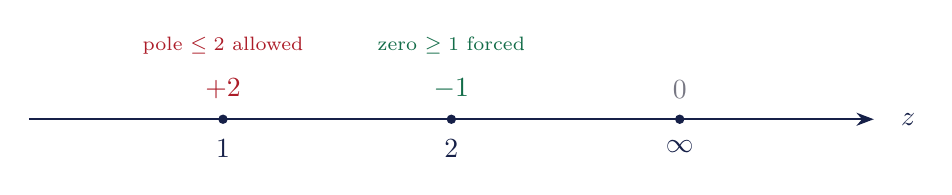
\begin{tikzpicture}[x=1.45cm,y=1cm]
  \draw[inkblue, line width=0.9pt, -{Stealth[length=2.2mm]}] (-0.7,0) -- (6.7,0);
  \node[inkblue] at (7.0,0) {$z$};
  \foreach \px in {1,3,5}{\fill[inkblue] (\px,0) circle (1.7pt);}
  \node[inkblue, below=4pt] at (1,0) {$1$};
  \node[inkblue, below=4pt] at (3,0) {$2$};
  \node[inkblue, below=4pt] at (5,0) {$\infty$};
  \node[polered, above=4pt, font=\bfseries] at (1,0) {$+2$};
  \node[zerogreen, above=4pt, font=\bfseries] at (3,0) {$-1$};
  \node[faint, above=4pt] at (5,0) {$0$};
  \node[polered, font=\scriptsize, above=20pt] at (1,0) {pole $\le 2$ allowed};
  \node[zerogreen, font=\scriptsize, above=20pt] at (3,0) {zero $\ge 1$ forced};
\end{tikzpicture}
\end{center}

\noindent
Because \(\deg D=1>0\), the divisor should be linearly equivalent to a single
point. We prove this by exhibiting an explicit principal divisor.

\begin{computation}[{Linear equivalence \(D\sim[\infty]\)}]
Let
\[
  h(z)=\frac{(z-1)^2}{z-2}.
\]
We compute \(\divisor(h)\) point by point.
\begin{itemize}
  \item At \(z=1\): the numerator vanishes to order \(2\), nothing cancels, so
        \(\ord_1(h)=+2\).
  \item At \(z=2\): the denominator vanishes to order \(1\), so \(h\) has a
        simple pole and \(\ord_2(h)=-1\).
  \item At \(z=\infty\): substitute \(z=1/w\),
        \[
          h=\frac{(1/w-1)^2}{1/w-2}
           =\frac{(1-w)^2/w^2}{(1-2w)/w}
           =\frac{(1-w)^2}{w\,(1-2w)} .
        \]
        Near \(w=0\) the numerator tends to \(1\) while the denominator has a
        simple zero, so \(h\) has a simple pole and \(\ord_\infty(h)=-1\).
\end{itemize}
Hence
\[
  \divisor(h)=2[1]-[2]-[\infty],
\]
a degree-zero (principal) divisor, as it must be. Rearranging,
\[
  D-[\infty]=2[1]-[2]-[\infty]=\divisor(h),
\]
so
\[
  \boxed{\,D\sim[\infty]\,}.
\]
\end{computation}

\noindent
Consequently
\[
  \OO(D)\;\cong\;\OO([\infty])\;\cong\;\OO(1).
\]
Since \(h^0(\PP^1,\OO(d))=d+1\) for \(d\ge0\), this already \emph{predicts} the
answer of the next section before we compute it:
\[
  \dim_{\CC}L(D)=h^0\bigl(\PP^1,\OO(1)\bigr)=2 .
\]

%=====================================================================
\section{Compute \(L(D)\) Completely}
%=====================================================================
\begin{definition}
\[
  L(D)=\bigl\{\,f\in\CC(z)\;:\;\divisor(f)+D\ge 0\,\bigr\}.
\]
\end{definition}

\noindent
For \(D=2[1]-[2]\) the single inequality \(\divisor(f)+D\ge0\) unpacks, point by
point, into:
\[
  \ord_1(f)\ge -2,\qquad
  \ord_2(f)\ge +1,
\]
\[
  \ord_p(f)\ge 0 \quad\text{for every finite } p\neq 1,2,
  \qquad
  \ord_\infty(f)\ge 0 .
\]
In words: \(f\) may carry \emph{at most a double pole} at \(z=1\), it
\emph{must vanish at least once} at \(z=2\), and it may have \emph{no other
pole anywhere}, the point \(\infty\) included.

\medskip
\noindent\textbf{Deriving the general form.}
Write \(f=P/Q\) in lowest terms.
\begin{itemize}
  \item The only pole permitted is at \(z=1\) of order \(\le2\), so the
        denominator is \(Q=(z-1)^2\) (taking the largest allowed pole; smaller
        ones are special cases).
  \item The forced zero at \(z=2\) means \((z-2)\mid P\).
  \item Holomorphy at \(\infty\) requires \(\ord_\infty(f)\ge0\), i.e.
        \(\deg P\le\deg Q=2\).
\end{itemize}
Therefore \(P=(z-2)(az+b)\) with \(a,b\in\CC\), and
\[
  \boxed{\;f(z)=\frac{(z-2)(az+b)}{(z-1)^2}\;}.
\]
The numerator has degree at most \(2\), matching the denominator's degree \(2\);
hence \(f\) tends to the finite value \(a\) as \(z\to\infty\) and has \emph{no}
pole at infinity. The two free parameters \(a,b\) confirm \(\dim_\CC L(D)=2\),
exactly as predicted.

\medskip
\noindent
Choosing the basis \(\{az+b\}=\{1,\;z-1\}\) of linear polynomials gives
\[
  L(D)=\operatorname{span}_{\CC}
  \left\{\,
    \frac{z-2}{(z-1)^2},\;
    \frac{z-2}{z-1}
  \,\right\}.
\]
Set
\[
  s_0=\frac{z-2}{(z-1)^2},
  \qquad
  s_1=\frac{z-2}{z-1}.
\]

\begin{center}
\renewcommand{\arraystretch}{1.7}
\setlength{\tabcolsep}{6pt}
\begin{tabular}{|>{\centering\arraybackslash}m{2.4cm}|c|c|c|c|}
\hline
\textbf{section} & \textbf{at }$z=1$ & \textbf{at }$z=2$
                 & \textbf{at }$\infty$ & \textbf{allowed by }$D$?\\
\hline
$\displaystyle s_0=\frac{z-2}{(z-1)^2}$
  & \textcolor{polered}{pole, order $2$}
  & \textcolor{zerogreen}{zero, order $1$}
  & zero, order $1$
  & \textcolor{zerogreen}{yes}\\
\hline
$\displaystyle s_1=\frac{z-2}{z-1}$
  & \textcolor{polered}{pole, order $1$}
  & \textcolor{zerogreen}{zero, order $1$}
  & unit (value $1$)
  & \textcolor{zerogreen}{yes}\\
\hline
\end{tabular}
\end{center}

\noindent
As a sanity check, \(\divisor(s_0)+D=\bigl([2]+[\infty]-2[1]\bigr)+\bigl(2[1]-[2]\bigr)=[\infty]\ge0\),
and \(\divisor(s_1)+D=\bigl([2]-[1]\bigr)+\bigl(2[1]-[2]\bigr)=[1]\ge0\).
Both lie in \(L(D)\).

%=====================================================================
\section{Translate \(L(D)\) into \(H^0(\PP^1,\OO(D))\)}
%=====================================================================
The divisor sheaf is defined on each open \(U\subseteq\PP^1\) by
\[
  \OO(D)(U)=\bigl\{\,f\in\MM(U)\;:\;\divisor(f)+D|_U\ge0\,\bigr\},
\]
where \(\MM\) is the sheaf of meromorphic functions. Taking global sections
collapses this to exactly the Riemann--Roch space:
\[
  H^0(\PP^1,\OO(D))=\OO(D)(\PP^1)=L(D).
\]

\philobox{A global section of \(\OO(D)\) is a meromorphic function whose bad
behavior is exactly compensated by the divisor \(D\).}

\noindent
The divisor \(D\) is thus a \emph{local rulebook}: at each point it permits
certain poles and demands certain zeros, and \(H^0\) collects precisely those
global meromorphic functions that obey every clause of the rulebook at once.

%=====================================================================
\section{Cartier Divisor Data}
%=====================================================================
Cover \(\PP^1\) by the three opens
\[
  U_0=\PP^1\setminus\{1,2\},\qquad
  U_1=\{\,|z-1|<r\,\},\qquad
  U_2=\{\,|z-2|<r\,\},
\]
with \(r<1\) small enough that \(U_1\) excludes \(2\) and \(U_2\) excludes \(1\)
(and the disks meet, if at all, only away from both \(1\) and \(2\)). Choose
local equations
\[
  f_0=1,\qquad f_1=(z-1)^2,\qquad f_2=(z-2)^{-1}.
\]
Each \(f_i\) cuts out \(D\) on its own patch:
\[
  \divisor(f_1)=2[1]\ \text{ near }1,\qquad
  \divisor(f_2)=-[2]\ \text{ near }2,\qquad
  \divisor(f_0)=0\ \text{ away from }1,2 .
\]
This is the defining feature of a \textbf{Cartier divisor}: the local data are
glued compatibly, meaning the ratios are holomorphic and nowhere zero on
overlaps,
\[
  \frac{f_i}{f_j}\in\OO^\times(U_i\cap U_j).
\]
Local meromorphic equations for the same divisor can differ only by holomorphic
units once the special points have been removed from the overlap.

%=====================================================================
\section{From Cartier Data to \(\OO(D)\)}
%=====================================================================
The sheaf \(\OO(D)\) is locally free of rank one, trivialized on each patch by
the inverse of the local equation:
\[
  \OO(D)\big|_{U_i}=f_i^{-1}\,\OO_{U_i},
  \qquad
  e_i:=f_i^{-1}\ \text{the local generator.}
\]
On an overlap the two generators are proportional,
\[
  e_i=f_i^{-1}=\frac{f_j}{f_i}\,f_j^{-1}=\frac{f_j}{f_i}\,e_j,
\]
so with the convention
\[
  g_{ij}=\frac{f_j}{f_i}
\]
we read off the transition functions:
\[
  g_{10}=\frac{f_0}{f_1}=\frac{1}{(z-1)^2},
  \qquad
  g_{20}=\frac{f_0}{f_2}=z-2,
\]
\[
  g_{12}=\frac{f_2}{f_1}=\frac{(z-2)^{-1}}{(z-1)^2}=\frac{1}{(z-2)(z-1)^2}.
\]
Each is a holomorphic unit on its overlap precisely because the offending
point has been removed:
\begin{itemize}
  \item \(g_{10}\) is a unit on \(U_1\cap U_0\) since \(z=1\notin U_0\);
  \item \(g_{20}\) is a unit on \(U_2\cap U_0\) since \(z=2\notin U_0\);
  \item \(g_{12}\) is a unit on \(U_1\cap U_2\) since \(z=1,2\notin U_1\cap U_2\)
        (the disks were chosen small and disjoint from each other's center).
\end{itemize}
They satisfy the cocycle identity \(g_{ij}g_{jk}=g_{ik}\); for instance
\(g_{10}\,g_{02}=\dfrac{f_0}{f_1}\cdot\dfrac{f_2}{f_0}=\dfrac{f_2}{f_1}=g_{12}\).

%=====================================================================
\section{Interpret \(\OO(D)\) as a Holomorphic Line Bundle}
%=====================================================================
The same data may be read geometrically. Glue the trivial line bundles
\[
  U_i\times\CC
\]
along the overlaps by declaring \((z,\,v_j)\in U_j\times\CC\) and
\((z,\,v_i)\in U_i\times\CC\) to be the same point whenever
\(v_i=g_{ij}\,v_j\). The result is a holomorphic line bundle whose sheaf of
holomorphic sections is exactly \(\OO(D)\):
\begin{center}
\(\OO(D)\) \emph{is obtained by gluing the trivial bundles }
\(U_i\times\CC\)\emph{ using the transition functions } \(g_{ij}\).
\end{center}
The invertible sheaf and the holomorphic line bundle are two languages for one
object.

\[
\begin{tikzcd}[row sep=large, column sep=huge]
\{(U_i,f_i)\}
   \arrow[r, "g_{ij}=f_j/f_i"]
   \arrow[d, "f_i^{-1}\OO_{U_i}"']
& \{g_{ij}\}\in Z^1(\mathfrak U,\OO^\times)
   \arrow[d, "\text{glue }U_i\times\CC"] \\
\OO(D)
   \arrow[r, "\sim"']
& \text{holomorphic line bundle }L_D
   \arrow[r, "{D\sim[\infty]}"]
& \OO(1)
\end{tikzcd}
\]

\begin{remark}
The cocycle \(\{g_{ij}\}\) defines a class in
\(H^1(\PP^1,\OO^\times)=\Pic(\PP^1)\cong\mathbb Z\), and that integer is
\(\deg D=1\). This is the cohomological face of the computation
\(D\sim[\infty]\): both say
\[
  \OO(D)\cong\OO(1),
\]
the unique degree-one line bundle on \(\PP^1\), which is moreover very ample
since \(\deg D=1\ge 2g+1=1\) for \(g=0\).
\end{remark}

%=====================================================================
\section{Interpret the Basis as Global Sections}
%=====================================================================
A global section \(s\in H^0(\PP^1,\OO(D))\) is represented on the patch \(U_i\)
by the \emph{holomorphic} function
\[
  a_i=f_i\,s .
\]
We compute the local representatives of \(s_0\) and \(s_1\).

\medskip
\noindent\textbf{Near \(z=1\)} (using \(f_1=(z-1)^2\)):
\[
  f_1 s_0=(z-1)^2\cdot\frac{z-2}{(z-1)^2}=z-2,
  \qquad
  f_1 s_1=(z-1)^2\cdot\frac{z-2}{z-1}=(z-1)(z-2).
\]
Both are holomorphic near \(z=1\); their values there are \(-1\) and \(0\).

\medskip
\noindent\textbf{Near \(z=2\)} (using \(f_2=(z-2)^{-1}\)):
\[
  f_2 s_0=(z-2)^{-1}\cdot\frac{z-2}{(z-1)^2}=\frac{1}{(z-1)^2},
  \qquad
  f_2 s_1=(z-2)^{-1}\cdot\frac{z-2}{z-1}=\frac{1}{z-1}.
\]
Both are holomorphic near \(z=2\); their values there are \(1\) and \(1\).

\warnbox{\textbf{Essential warning.}
The raw meromorphic functions \(s_0\) and \(s_1\) both vanish at \(z=2\), but the
corresponding global sections do \emph{not} vanish simultaneously there. Indeed
their honest local values at \(z=2\), read in the \(U_2\)-trivialization, are
\(f_2 s_0\big|_{2}=1\) and \(f_2 s_1\big|_{2}=1\) --- both nonzero. A section of
\(\OO(D)\) must be evaluated only \emph{after} choosing a local trivialization;
the naive number \(s_i(2)=0\) is an artifact of the chart \(f_0=1\), not a
property of the section.}

%=====================================================================
\section{Compute the Projective Map}
%=====================================================================
The basis \((s_0,s_1)\) of \(H^0(\PP^1,\OO(D))\) determines a map
\[
  \Phi_D:\PP^1\longrightarrow\PP^1,
  \qquad
  p\longmapsto[\,s_0(p):s_1(p)\,],
\]
\emph{interpreted through local trivializations}: at each point one divides by
the local generator before forming homogeneous coordinates.

\medskip
\noindent\textbf{On \(U_0\)} (\(f_0=1\), so the trivialization is the identity):
\[
  \Phi_D(z)=\left[\frac{z-2}{(z-1)^2}:\frac{z-2}{z-1}\right].
\]
For \(z\neq1,2\) we may clear the common factor \(\dfrac{z-2}{z-1}\) and then
the factor \((z-1)\):
\[
  \left[\frac{z-2}{(z-1)^2}:\frac{z-2}{z-1}\right]
  =\left[\frac{1}{z-1}:1\right]
  =[\,1:z-1\,].
\]

\noindent\textbf{At \(z=2\)} (use the \(U_2\)-trivialization \(f_2=(z-2)^{-1}\)):
\[
  \Phi_D(2)=\bigl[\,f_2 s_0:f_2 s_1\,\bigr]_{z=2}
  =\left[\frac{1}{(2-1)^2}:\frac{1}{2-1}\right]=[\,1:1\,],
\]
matching \([\,1:z-1\,]\big|_{z=2}=[1:1]\). The point \(z=2\) is therefore
\emph{not} a base point.

\medskip
\noindent\textbf{At \(z=1\)} (use the \(U_1\)-trivialization \(f_1=(z-1)^2\)):
\[
  \Phi_D(1)=\bigl[\,f_1 s_0:f_1 s_1\,\bigr]_{z=1}
  =\bigl[\,(z-2):(z-1)(z-2)\,\bigr]_{z=1}
  =[-1:0]=[\,1:0\,],
\]
matching \([\,1:z-1\,]\big|_{z=1}=[1:0]\).

\medskip
\noindent\textbf{At \(z=\infty\):} from \(\Phi_D(z)=[\,1:z-1\,]=\bigl[\tfrac{1}{z-1}:1\bigr]\),
\[
  \Phi_D(\infty)=\lim_{z\to\infty}\Bigl[\tfrac{1}{z-1}:1\Bigr]=[\,0:1\,].
\]

\noindent
Collecting every chart,
\[
  \boxed{\;\Phi_D(z)=[\,1:z-1\,]\;}.
\]
In homogeneous coordinates \(z=X/Y\) one has
\(\,[\,1:z-1\,]=[\,1:\tfrac{X-Y}{Y}\,]=[\,Y:X-Y\,]\), hence
\[
  \boxed{\;[X:Y]\longmapsto[\,Y:X-Y\,]\;}.
\]
The matrix \(\left(\begin{smallmatrix}0&1\\ 1&-1\end{smallmatrix}\right)\) has
determinant \(-1\neq0\), so \(\Phi_D\in\mathrm{PGL}_2(\CC)\) is a degree-one
\emph{automorphism} of \(\PP^1\). Equivalently, the complete linear system
\(|D|\) is base-point free and \(\OO(D)=\OO(1)\) is very ample, so \(\Phi_D\) is
an embedding --- here, an isomorphism onto all of \(\PP^1\).

%=====================================================================
\clearpage
\section{One-Page Conceptual Map}
%=====================================================================
\noindent
One divisor at the center; eight incarnations on the rim. The blue spokes are
the \emph{readings} of \(D\); the amber rim arrows are the \emph{translations}
between incarnations.

\bigskip
\begin{center}
\resizebox{\textwidth}{!}{%
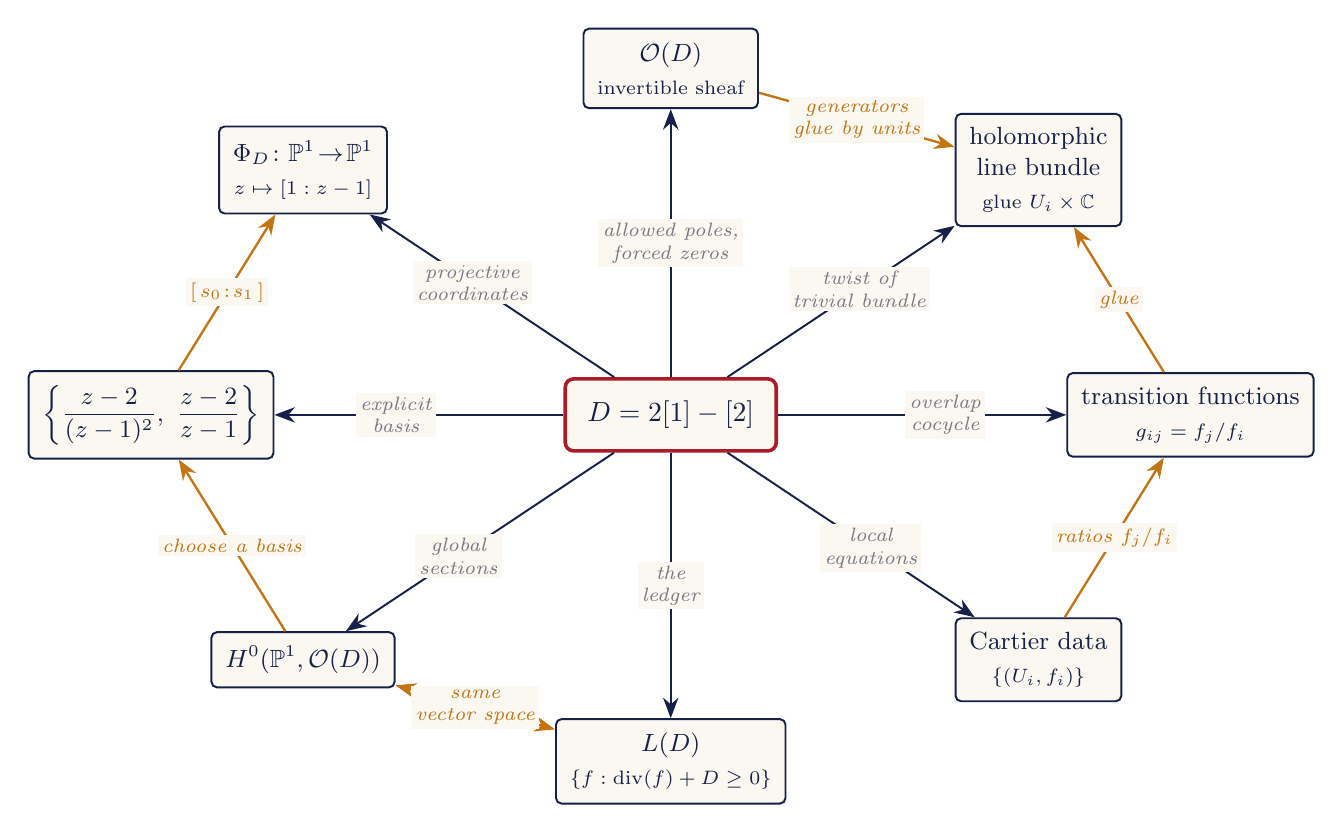
\begin{tikzpicture}
  % ---- nodes (drawn after we reserve coordinates) ----
  \node[centernode] (D)   at (0,0)        {$D=2[1]-[2]$};
  \node[mapnode] (OD)  at (0,4.4)         {$\OO(D)$\\[1pt]\scriptsize invertible sheaf};
  \node[mapnode] (BUN) at (4.67,3.11)     {holomorphic\\ line bundle\\[1pt]\scriptsize glue $U_i\times\CC$};
  \node[mapnode] (GIJ) at (6.6,0)         {transition functions\\[1pt]\scriptsize $g_{ij}=f_j/f_i$};
  \node[mapnode] (CAR) at (4.67,-3.11)    {Cartier data\\[1pt]\scriptsize $\{(U_i,f_i)\}$};
  \node[mapnode] (LD)  at (0,-4.4)        {$L(D)$\\[1pt]\scriptsize $\{f:\divisor(f)+D\ge0\}$};
  \node[mapnode] (H0)  at (-4.67,-3.11)   {$H^0(\PP^1,\OO(D))$};
  \node[mapnode] (BAS) at (-6.6,0)        {$\left\{\dfrac{z-2}{(z-1)^2},\ \dfrac{z-2}{z-1}\right\}$};
  \node[mapnode] (PHI) at (-4.67,3.11)    {$\Phi_D\colon\PP^1\!\to\!\PP^1$\\[1pt]\scriptsize $z\mapsto[1:z-1]$};

  % ---- spokes: D -> incarnations ----
  \draw[maparrow] (D) -- node[arrlbl]{allowed poles,\\ forced zeros} (OD);
  \draw[maparrow] (D) -- node[arrlbl,pos=0.58]{twist of\\ trivial bundle} (BUN);
  \draw[maparrow] (D) -- node[arrlbl,pos=0.58]{overlap\\ cocycle} (GIJ);
  \draw[maparrow] (D) -- node[arrlbl,pos=0.58]{local\\ equations} (CAR);
  \draw[maparrow] (D) -- node[arrlbl]{the\\ ledger} (LD);
  \draw[maparrow] (D) -- node[arrlbl,pos=0.58]{global\\ sections} (H0);
  \draw[maparrow] (D) -- node[arrlbl,pos=0.58]{explicit\\ basis} (BAS);
  \draw[maparrow] (D) -- node[arrlbl,pos=0.58]{projective\\ coordinates} (PHI);

  % ---- rim: translations between incarnations ----
  \draw[rimarrow] (CAR) -- node[rimlbl]{ratios $f_j/f_i$} (GIJ);
  \draw[rimarrow] (GIJ) -- node[rimlbl]{glue} (BUN);
  \draw[rimarrow] (OD)  -- node[rimlbl]{generators\\ glue by units} (BUN);
  \draw[rimarrow,{Stealth[length=2.6mm]}-{Stealth[length=2.6mm]}]
        (LD) -- node[rimlbl]{same\\ vector space} (H0);
  \draw[rimarrow] (H0)  -- node[rimlbl]{choose a basis} (BAS);
  \draw[rimarrow] (BAS) -- node[rimlbl]{$[\,s_0\!:\!s_1\,]$} (PHI);
\end{tikzpicture}}
\end{center}

\bigskip
\noindent\small
Sample readings of the labels:
\(D\to\OO(D)\): allowed poles and forced zeros become a sheaf.\quad
\(\OO(D)\to\) line bundle: local generators glue by units.\quad
\(H^0(\OO(D))\leftrightarrow L(D)\): global sections are meromorphic functions
obeying \(D\).
\clearpage

%=====================================================================
\section*{Visual Design: The Divisor as a Wall of Computation}
\addcontentsline{toc}{section}{Visual Design: The Divisor as a Wall of Computation}
%=====================================================================
Imagine this page not as clean typeset exposition but as the chalk-and-ink wall
of an old mathematician mid-thought. The divisor sits boxed at the center.
Around \(z=1\) a \textbf{double spiral} coils outward --- a pole of order two,
two sheets winding away from the point. Around \(z=2\) a \textbf{dark sink}
swallows the neighborhood, arrows pressing inward toward a forced zero. From
the central box, hand-drawn arrows shoot toward the Cartier data, the sheaf, the
line bundle, the global sections, and the projective map, while the margins are
scrawled with the working formulas. It is not polished exposition, but the
wall-writing of someone conquering abstraction by explicit computation.

\bigskip
\begin{center}
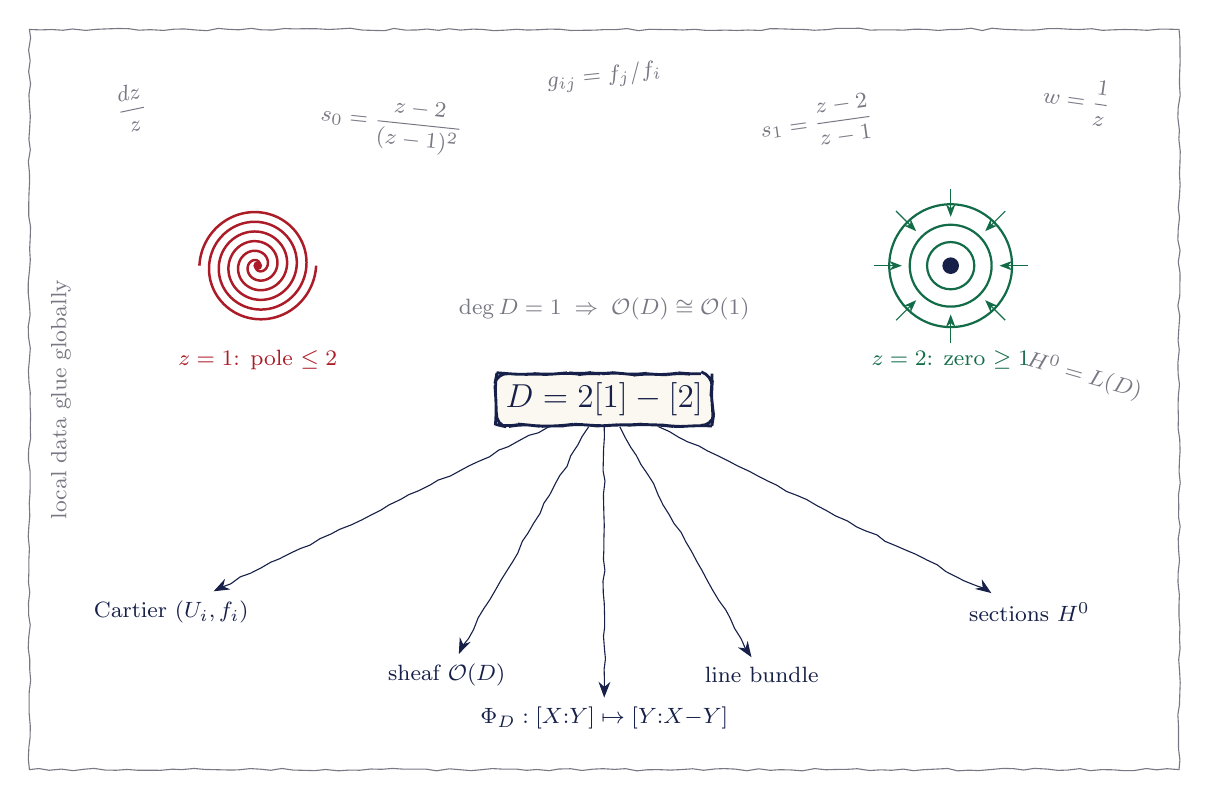
\begin{tikzpicture}[scale=1]
  % rough frame
  \draw[faint, pencil, line width=0.4pt] (-7.3,-4.7) rectangle (7.3,4.7);

  % central boxed divisor
  \node[draw=inkblue, pencil, line width=1pt, fill=paper, rounded corners,
        font=\large\bfseries, text=inkblue] (D) at (0,0) {$D=2[1]-[2]$};

  % ---- pole of order 2 at z=1 : double spiral (left) ----
  \begin{scope}[shift={(-4.4,1.7)}]
     \draw[polered, line width=0.9pt]
        plot[domain=0:1080,samples=200,smooth]
        ({0.00068*\x*cos(\x)},{0.00068*\x*sin(\x)});
     \draw[polered, line width=0.9pt]
        plot[domain=0:1080,samples=200,smooth]
        ({0.00068*\x*cos(\x+180)},{0.00068*\x*sin(\x+180)});
     \fill[polered] (0,0) circle (1.6pt);
     \node[polered, font=\footnotesize] at (0,-1.2) {$z=1$: pole $\le 2$};
  \end{scope}

  % ---- forced zero at z=2 : dark sink (right) ----
  \begin{scope}[shift={(4.4,1.7)}]
     \draw[zerogreen, line width=0.8pt] (0,0) circle (0.78);
     \draw[zerogreen, line width=0.8pt] (0,0) circle (0.52);
     \draw[zerogreen, line width=0.8pt] (0,0) circle (0.30);
     \fill[inkblue] (0,0) circle (3pt);
     \foreach \a in {0,45,...,315}{
        \draw[zerogreen,-{Stealth[length=1.6mm]}] (\a:0.98) -- (\a:0.62);}
     \node[zerogreen, font=\footnotesize] at (0,-1.2) {$z=2$: zero $\ge 1$};
  \end{scope}

  % ---- radiating hand-drawn arrows to labels ----
  \node[inkblue, font=\footnotesize] (cart) at (-5.5,-2.7) {Cartier $(U_i,f_i)$};
  \node[inkblue, font=\footnotesize] (sheaf)at (-2.0,-3.5) {sheaf $\OO(D)$};
  \node[inkblue, font=\footnotesize] (bndl) at ( 2.0,-3.5) {line bundle};
  \node[inkblue, font=\footnotesize] (sect) at ( 5.4,-2.7) {sections $H^0$};
  \node[inkblue, font=\footnotesize] (map)  at ( 0,-4.05)
        {$\Phi_D:[X{:}Y]\mapsto[Y{:}X{-}Y]$};

  \draw[inkblue, pencil, -{Stealth[length=2mm]}] (D) -- (cart);
  \draw[inkblue, pencil, -{Stealth[length=2mm]}] (D) -- (sheaf);
  \draw[inkblue, pencil, -{Stealth[length=2mm]}] (D) -- (bndl);
  \draw[inkblue, pencil, -{Stealth[length=2mm]}] (D) -- (sect);
  \draw[inkblue, pencil, -{Stealth[length=2mm]}] (D) -- (map);

  % ---- marginal graffiti ----
  \node[faint, rotate=12,  font=\footnotesize] at (-6.0,3.7)  {$\dfrac{dz}{z}$};
  \node[faint, rotate=-8,  font=\footnotesize] at ( 6.0,3.8)  {$w=\dfrac1z$};
  \node[faint, rotate=-16, font=\footnotesize] at ( 6.1,0.3)  {$H^0=L(D)$};
  \node[faint, rotate=90,  font=\footnotesize] at (-6.9,0)    {local data glue globally};
  \node[faint, rotate=6,   font=\footnotesize] at ( 0,4.1)    {$g_{ij}=f_j/f_i$};
  \node[faint, rotate=-6,  font=\footnotesize] at (-2.7,3.5)  {$s_0=\dfrac{z-2}{(z-1)^2}$};
  \node[faint, rotate=8,   font=\footnotesize] at ( 2.7,3.5)  {$s_1=\dfrac{z-2}{z-1}$};
  \node[faint, rotate=0,   font=\footnotesize] at ( 0,1.15)   {$\deg D=1\;\Rightarrow\;\OO(D)\cong\OO(1)$};
\end{tikzpicture}
\end{center}

%=====================================================================
\section*{Final Reflection}
\addcontentsline{toc}{section}{Final Reflection}
%=====================================================================
\philobox{%
So the formal sum \(D=2[1]-[2]\) was never merely formal. Held to the light it
is at once a ledger of one forced zero and one bounded pole; a triple of Cartier
local equations \((1,\,(z-1)^2,\,(z-2)^{-1})\); an invertible sheaf \(\OO(D)\);
a holomorphic line bundle glued from the units \(\tfrac{1}{(z-1)^2}\) and
\(z-2\); a two-dimensional space of global meromorphic functions spanned by
\(s_0\) and \(s_1\); and the pair of projective coordinates that realize
\(\PP^1\) as itself through \([X:Y]\mapsto[Y:X-Y]\). Abstraction did not have to
be believed --- it had to be \emph{computed}. Local data, gluing, global
sections, and projective geometry were all already folded inside three symbols
and a difference. That is the quiet violence of a divisor: a single line of
notation that, interrogated by calculation, opens into the entire architecture
of a curve.}

\end{document}
